%---------------------------------------------------------------------%
%  LaTeX Course Notes Template                                        %
%                                                                     %
%  Copyright (C) 2012 Zev Chonoles                                    %
%  zevchonoles@gmail.com                                              %
%  http://math.uchicago.edu/~chonoles/                                %
%                                                                     %
%  Please leave this information in the source code as                %
%  attribution if you choose to edit or redistribute this file.       %
%                                                                     %
%  This work is licensed under the Creative Commons Attribution-      %
%  ShareAlike 3.0 Unported License. To view a copy of this license,   %
%  visit http://creativecommons.org/licenses/by-sa/3.0/.              %
%                                                                     %
%---------------------------------------------------------------------%

\documentclass[11pt]{article}






%----------%
%  Basics  %
%----------%


%  Specfies basic information.
%  In the metadata section of the preamble, you can specify the subject and a list of keywords for the PDF.
%
\newcommand{\coursetitle}{Math 500 - Topology and Geometry}
\newcommand{\lecturer}{Brian Weber}
\newcommand{\notetaker}{Zach Schutzman}
\newcommand{\notetakersemail}{ianzach+notes@seas.upenn.edu}
\newcommand{\courseterm}{Fall 2017}
\newcommand{\institution}{University of Pennsylvania}


%  array provides more column styles for the tabular and array environments.
%  (http://ctan.org/pkg/array)
%
%  parskip sets block paragraphs as the default, instead of indentation.
%  (http://www.ctan.org/pkg/parskip)
%
\usepackage[margin=1in]{geometry}
\usepackage{amsmath,amssymb,amsthm,amsfonts,array,parskip}


%  Allows equation, align, gather, etc. environments to split across pages.
\allowdisplaybreaks


%  Sets date formatting to the ISO 8601 standard, YYYY-MM-DD.
\usepackage{datetime} \renewcommand{\dateseparator}{-} \yyyymmdddate






%---------%
%  Fonts  %
%---------%


%  Defines \cal for standard calligraphy, \eucal for Euler calligraphy, and \frak for Fraktur.
\usepackage{eucal}  \let\eucal\mathcal  \let\cal\CMcal  \renewcommand{\frak}{\mathfrak}


%  Removes ligatures (e.g. the connection ordinarily made between the two f's in "differentiable").
\usepackage{microtype} \DisableLigatures{encoding=*,family=*}


%  Removes extra space after periods.




%-------------------------------%
%  Environments and Sectioning  %
%-------------------------------%


%  Defines some standard theorem environments, in both numbered and non-numbered versions. The numbering of each enviroment will be reset for each lecture.
\newcounter{lecture}       \setcounter{lecture}{0}
\newcounter{tN}[lecture]   \newcounter{dN}[lecture]
\newcounter{lN}[lecture]   \newcounter{rN}[lecture]
\newcounter{cN}[lecture]   \newcounter{eN}[lecture]
\newcounter{pN}[lecture]
\newcounter{clN}[lecture]

\newtheorem*{theorem}{Theorem}          \newtheorem{theorem-N}[tN]{Theorem}
\newtheorem*{lemma}{Lemma}              \newtheorem{lemma-N}[lN]{Lemma}
\newtheorem*{corollary}{Corollary}      \newtheorem{corollary-N}[cN]{Corollary}
\newtheorem*{proposition}{Proposition}  \newtheorem{proposition-N}[pN]{Proposition}

\theoremstyle{definition}
\newtheorem*{definition}{Definition}    \newtheorem{definition-N}[dN]{Definition}
\newtheorem*{remark}{Remark}            \newtheorem{remark-N}[rN]{Remark}
\newtheorem*{example}{Example}          \newtheorem{example-N}[eN]{Example}


\newtheorem*{claim}{Claim}    \newtheorem{claim-N}[clN]{Claim}


%  Modifies the spacing above theorem environments, which is messed up when using the parskip package.
%  (http://tex.stackexchange.com/questions/22119)
%
\makeatletter \def\thm@space@setup{\thm@preskip=\parskip \thm@postskip=0pt} \makeatother


%  Modifies the spacing above the proof environment.
%  (http://tex.stackexchange.com/questions/49801)
%
\makeatletter \renewenvironment{proof}[1][\proofname]{\pushQED{\qed}\normalfont
	\partopsep=\z@skip \topsep=\z@skip \trivlist \item[\hskip\labelsep\itshape #1\@addpunct{.}]
	\ignorespaces}{\popQED\endtrivlist\@endpefalse} \makeatother


%  Removes extra space before and after section headings.
\usepackage[compact]{titlesec}






%-------------------------%
%  Pictures and Diagrams  %
%-------------------------%


%  Allows for the use of colors.
%  (http://www.ctan.org/pkg/xcolor)
%
\usepackage[usenames,dvipsnames]{xcolor}
\definecolor{myred}{rgb}{0.9,0.2,0.2}
\definecolor{mygreen}{rgb}{0.2,0.6,0.2}
\definecolor{myblue}{rgb}{0.2,0.2,0.8}


%  graphicx provides advanced graphics options.
%  (http://ctan.org/pkg/graphicx)
%
\usepackage{graphicx}


%  tikz is for drawing all sorts of pictures and diagrams.
%  tikz-cd makes creating commutative diagrams in tikz a bit easier.
%  (http://www.ctan.org/pkg/pgf)
%  (http://www.ctan.org/pkg/tikz-cd)
%
\usepackage{tikz}
\usepackage{tikz-cd}
\usepackage{pgf,pgfplots}
\usetikzlibrary{arrows,calc,decorations,decorations.markings,fadings,positioning,patterns,shapes}
\tikzset{>=latex}
\tikzstyle{mypoint}=[inner sep=0pt,outer sep=0pt,minimum size=5pt,fill,circle]


\definecolor{ttqqqq}{rgb}{0.2,0.,0.}
\definecolor{ffffff}{rgb}{1.,1.,1.}
%\usetikzlibrary{external}
%\tikzexternalize



%------------------------%
%  Commands and Symbols  %
%------------------------%


%  Creates commands by running over a comma-separated list. For example,
%
%     \forcsvlist{\define{\newcommand}{\textbf}{bold}}{A,B}
%
%  would create
%
%     \newcommand{\boldA}{\textbf{A}}    \newcommand{\boldB}{\textbf{B}}
%
%  (http://tex.stackexchange.com/a/5776/20882)
%
\usepackage{etoolbox}
\newcommand{\define}[4]{\expandafter#1\csname#3#4\endcsname{#2{#4}}}
\forcsvlist{\define{\DeclareMathOperator}{}{}}{im,coker,rad,nil,Ann,Ass,codim,Spec,mSpec,diam,ord,Supp,supp,disc,Ob,vol,rank,Sym,Alt,Ind}
\forcsvlist{\define{\newcommand}{\mathrm}{}}{Hom,Mor,id,GL,SL,SO,SU,U,M,Mat,Ext,Tor,Res,Cor,Inf,End,Irr,Aut,Gal,lcm,tr,sign,triv,diag,Map,op,ev,act,alg,sep,unr,nr,ab}

%  Creates commands for some names of categories in the sans-serif font.
\forcsvlist{\define{\newcommand}{\mathsf}{}}{Set,Grp,Ab,CRing,Mod,Vect,Cat,Top,PreSh,Sh,Sch,Nat,Fun,Diff}

%  Creates commands for some blackboard bold letters.
\forcsvlist{\define{\newcommand}{\mathbb}{}}{N,Z,Q,R,C,F,G,T,A,B,D}


%  Saves the section symbol, paragraph symbol, Hungarian accent, and Scandanavian O in the macros \SS, \PP, \HH, and \OO, then redefines \S, \P, \H, and \O to be the corresponding blackboard bold letters.
%
\let\SS\S  \let\PP\P  \let\HH\H  \let\OO\O
\forcsvlist{\define{\renewcommand}{\mathbb}{}}{S,P,H,O}


%  latexsym defines some alternative versions of amssymb symbols.
%  (http://www.bakoma-tex.com/doc/latex/base/latexsym.pdf)
%
\usepackage{latexsym}


%  Defines a copyright symbol that is a bit nicer than the built-in one.
\newcommand{\mycopyrightsymbol}{\raisebox{-0.3ex}{\tikz{\node[inner sep=0pt,outer sep=0pt] at (0,0) {\textsc{c}};\draw (0,0) circle (0.18);}}}


%  Defines commands for real and complex projective space.
\newcommand{\RP}{\mathbb{R}\mathrm{P}}  \newcommand{\CP}{\mathbb{C}\mathrm{P}}


%  Defines a bordered matrix with square bracket delimiters instead of parentheses.
%  (http://tex.stackexchange.com/questions/55054)
%
\let\bbordermatrix\bordermatrix
\patchcmd{\bbordermatrix}{8.75}{4.75}{}{}
\patchcmd{\bbordermatrix}{\left(}{\left[}{}{}
\patchcmd{\bbordermatrix}{\right)}{\right]}{}{}


%  Calls one of the mathabx font families so that it is possible to use its symbols without making a global change.
%  (http://www.ctan.org/pkg/mathabx)
%  (http://tex.stackexchange.com/questions/14386)
%
\DeclareFontFamily{U}{mathb}{\hyphenchar\font45}
\DeclareFontShape{U}{mathb}{m}{n}{<5> <6> <7> <8> <9> <10> gen * mathb
	<10.95> mathb10 <12> <14.4> <17.28> <20.74> <24.88> mathb12}{}
\DeclareSymbolFont{mathb}{U}{mathb}{m}{n}


%  Defines circular arrows.
\DeclareMathSymbol{\lcirclearrow}{0}{mathb}{'366}
\DeclareMathSymbol{\rcirclearrow}{0}{mathb}{'367}
\newcommand{\leftcirclearrow}{\mathrel{\ensuremath{\raisebox{0.1ex}{\scalebox{0.9}{\rotatebox[origin=c]{90}{$\lcirclearrow$}}}}}}
\newcommand{\rightcirclearrow}{\mathrel{\ensuremath{\raisebox{0.1ex}{\scalebox{0.9}{\rotatebox[origin=c]{270}{$\rcirclearrow$}}}}}}


%  Gives semantic names for some common math symbols.
\newcommand{\iso}{\cong}
\newcommand{\htop}{\sim}
\newcommand{\htopequiv}{\simeq}
\newcommand{\cupprod}{\mathbin{\smallsmile}}
\newcommand{\capprod}{\mathbin{\smallfrown}}
\newcommand{\wedgesum}{\mathbin{\vee}}
\newcommand{\boundary}{\partial}
\renewcommand{\emptyset}{\varnothing}
\newcommand{\characteristic}{\mathrm{char}}
\newcommand{\symdiff}{\mathbin{\vartriangle}}
\newcommand{\convolute}{\mathbin{\ast}}
\newcommand{\actson}{\rightcirclearrow}
\newcommand{\actedonby}{\leftcirclearrow}
\newcommand{\directsum}{\oplus}
\newcommand{\bigdirectsum}{\bigoplus}
\newcommand{\tensor}{\otimes}
\newcommand{\bigtensor}{\bigotimes}
\newcommand{\free}{\mathbin{\ast}}
\newcommand{\bigfree}{\mathop{\ensuremath{\raisebox{-0.7ex}{\scalebox{2.3}{$\ast$}}}}}
\renewcommand{\complement}[1]{{#1}^{\mathsf{c}}}
\newcommand{\transpose}[1]{{#1}^{\textsf{T}}}
\newcommand{\union}{\cup}
\newcommand{\intersect}{\cap}
\newcommand{\transverse}{\mathrel{\raisebox{1.1ex}{$-$}\mathllap{\pitchfork\hspace{0.22mm}}}}



\def\multiset#1#2{\ensuremath{\left(\kern-.3em\left(\genfrac{}{}{0pt}{}{#1}{#2}\right)\kern-.3em\right)}}



%-----------------------------------%
%  Things Specific to Course Notes  %
%-----------------------------------%


%  Formatting for the table of contents. The first line allows for multi-column environments, the second line removes the heading "Contents".
\usepackage{multicol} \setlength{\columnsep}{3cm}
\makeatletter \renewcommand\tableofcontents{\@starttoc{toc}} \makeatother


%  Sets the page style.
\usepackage{fancyhdr}
\pagestyle{fancy}
\renewcommand{\headrulewidth}{0pt}
\renewcommand{\footrulewidth}{0.5pt}
\setlength{\headheight}{14pt}
\lfoot{\parbox[t]{1in}{\centering Last edited\\ \today}}
\cfoot{\parbox[t]{3in}{\centering \coursetitle}}
\rfoot{\parbox[t]{0.9in}{\centering Page \thepage\\ Lecture \arabic{lecture}}}


%  Sets the inputs for \maketitle.
\author{%Lectures by \lecturer\\ 
	Notes by \notetaker}
\title{\coursetitle}
\date{\institution, \courseterm}


%  Defines headings for each day's notes.
\newcommand{\classheader}[1]{\stepcounter{lecture}\newpage\section*{Lecture \arabic{lecture} (#1)}
	\phantomsection \addcontentsline{toc}{section}{Lecture \arabic{lecture} (#1)}}


%---------------------------------------%
%  Miscellaneous Additions to Template  %
%---------------------------------------%

% http://tex.stackexchange.com/questions/18359
\pgfplotsset{compat=newest}

\newcommand{\Cinfty}{\ensuremath{C^{\infty}}}
\newcommand{\Crit}{\mathrm{Crit}}
\usepackage{mathtools}
\newcommand{\Or}{\mathrm{Or}}
\renewcommand{\Re}{\mathrm{Re}}
\renewcommand{\Im}{\mathrm{Im}}
\usepackage{mathrsfs}
\newtheorem*{examples}{Examples}
\newtheorem*{exercise}{Exercise}
\usepackage{pdfpages}
\newcommand{\Lie}{\mathrm{Lie}}
\newcommand{\Diffeo}{\mathrm{Diffeo}}

\newcommand{\connection}{\nabla}
\newcommand{\new}{\mathrm{new}}


\newcommand{\review}{{\huge\color{myred}{$\star$}}}


%---------------------------%
%  Hyperlinks and Metadata  %
%---------------------------%
%
% (this section must come last!)


%  hyperref enables for the creation of hyperlinks, and also specifies the metadata of the PDF file.
%  hyperxmp allows more metadata to be specified.
%  (http://www.ctan.org/pkg/hyperref)
%  (http://www.ctan.org/pkg/hyperxmp)
%  (http://tex.stackexchange.com/questions/41461)
%
\usepackage{hyperref}
\usepackage{hyperxmp}
\hypersetup{
	pdfauthor={\notetaker},
	pdftitle={\coursetitle},
	pdfproducer={LaTeX},
	%pdfcopyright={Copyright (C) \the\year\ \notetaker. This work is licensed under a Creative Commons Attribution-ShareAlike 3.0 Unported License. All attribution should be to \lecturer\ as the lecturer, and to \notetaker\ as the person taking these notes.},
	pdfsubject={differential topology},
	pdfkeywords={},
	%pdflicenseurl={http://creativecommons.org/licenses/by-sa/3.0/},
	colorlinks=true,
	linkcolor=myred,
	citecolor=mygreen,
	urlcolor=myblue,
	linktoc=page,
	pdfstartview=FitH
}






%------------%
%  Document  %
%------------%


\begin{document}
	
	
	%  The command
	%
	%  \thispagepdflabel{text}
	%
	%  sets the PDF page number (*not* the internal LaTeX page number) to be "text". This does not have to be a numeral; it could be a word, e.g. "Title". This lets one avoid the issue of having the PDF's page numbering not aligning with the page numbering LaTeX used in the document.
	%
	%  (http://tex.stackexchange.com/questions/85558)
	
	
	%  Title
	%
	\maketitle
	\thispdfpagelabel{Title}
	\thispagestyle{empty}
	\setcounter{page}{-1}
	\vspace{0.3in}
	
	
	
	%  Table of Contents
	%
	\begin{center}
		\begin{minipage}[t]{0.9\textwidth}
			\begin{multicols}{2}
				\tableofcontents
			\end{multicols}
		\end{minipage}
	\end{center}
	
	
	
	\newpage
	\thispdfpagelabel{-}
	\thispagestyle{empty}
	
	
	
	%  Introduction
	%
	\section*{Introduction}
	Math 500 is a Masters-level first-course in Topology and Geometry.  The course follows James Munkres' \textit{Topology, 2ed.} and this set of notes is based on the Fall 2017 offering.
	
	These notes are being live-TeXed, though I edit for typos and add diagrams requiring the Ti\textit{k}Z package separately. I am using the editor TeXstudio.  The template for these notes was created by Zev Chonoles and is made available (and being used here) under a Creative Commons License. 
	
	I am responsible for all faults in this document, mathematical or otherwise; any merits of the material here should be credited to the lecturer, not to me.
	
	Please email any corrections or suggestions to \expandafter\href{mailto:\notetakersemail}{\texttt{\notetakersemail}}.
	
	%\medskip
	%
	%\section*{Acknowledgments}
	%
	%Thank you to all of my fellow students who sent me suggestions and corrections, and who lent me their own notes from days I was absent. My notes are much improved due to your help.
	
	
	%%  Copyright
	%%
	%\section*{Copyright}
	%Copyright \mycopyrightsymbol\ 2012 \notetaker.
	%
	%This work is licensed under a Creative Commons Attribution-ShareAlike 3.0 Unported License. This means you are welcome to do essentially anything with this work, including editing, %adapting, distributing, and making commercial use of it, as long as you
	%\begin{itemize}
	%\item include an attribution of \lecturer\ as the lecturer of the course these notes are based on, and \notetaker\ as the person taking the notes,
	%\item do so in a way that does not suggest either of us endorses you or your use of this work, and
	%\item if you alter, transform, or build upon this work, you must apply to your work the same, or similar, license to this one.
	%\end{itemize}
	%More details are available at \href{https://creativecommons.org/licenses/by-sa/3.0/deed.en\_US}{\texttt{https://creativecommons.org/licenses/by-sa/3.0/deed.en\_US}}.
	
	\newpage
	
	
	%  Make a separate file for each lecture, for example, using a naming scheme like this:
	%
	%  lecture1.tex, lecture2.tex, ...
	%
	%  and keep them in the same folder as this main file. By doing it this way (instead of keeping all the notes in the main file), if you're only working on the notes for one lecture, you can easily comment out the lines corresponding to the other lectures.
	%
	
		
	\classheader{}
	
	\section*{What is Combinatorics?}
	
	Combinatorics is the mathematics of counting.  Suppose we have some $n\in\mathbb{N}$ and a set $S$ of objects which somehow depend on $n$.  Combinatorics addresses the question "How many objects are in $S$?"  More formally, this is a function $f: \mathbb{N}\rightarrow \mathbb{N}$ which counts the number of objects in $S$ as a function of $n$.  What do we know about $f$?
	
	\example{Let $S_1$ be the set of binary sequences of length $n$.  Then $f(n)=2^n$.}
	\example{Let $S_2$ be the symmetric group on $n$ elements.  Then $f(n)=n!$.}
	
	\definition{A \textbf{derangement} is a permutation in the symmetric group which has no fixed points.}  
	\example{The set of derangements on $n$ elements, $D_n = \{\sigma\in S_n |\  \sigma(k)\neq k \  \forall k\leq n\}$, has size  $\#D_n = n!\sum\limits_{i=0}^{n} \frac{(-i)^i}{n!}$. }
	
	\example{Suppose we have a $2\times n$ board, which we want to tile with $2\times 1$ dominoes.  How many different ways are there to do this?  If $S = \{proper \ domino \ tilings \ of \ a \ 2\times n \ board\}$, then we have $\#S=F_n$, the $n$th Fibonacci number.}
	
	
\begin{center}	
\begin{tikzpicture}[line cap=round,line join=round,>=triangle 45,x=1.0cm,y=1.0cm]
\clip(-6.08,-1.94) rectangle (9.52,7.2);
\fill[line width=2.pt,color=ffffff,fill=ffffff,fill opacity=1.0] (-3.2,5.42) -- (1.8,5.42) -- (1.8,3.68) -- (-3.2,3.68) -- cycle;
\draw [line width=2.pt] (-3.2,5.42)-- (1.8,5.42);
\draw [line width=2.pt,color=ttqqqq] (-3.2,5.42)-- (1.8,5.42);
\draw [line width=2.pt,color=ttqqqq] (1.8,5.42)-- (1.8,3.68);
\draw [line width=2.pt,color=ttqqqq] (1.8,3.68)-- (-3.2,3.68);
\draw [line width=2.pt,color=ttqqqq] (-3.2,3.68)-- (-3.2,5.42);
\draw [line width=2.pt] (-2.34,5.42)-- (-2.34,3.68);
\draw [line width=2.pt] (-1.5,5.42)-- (-1.5,3.68);
\draw [line width=2.pt] (0.96,5.42)-- (0.96,3.68);
\draw [line width=2.pt] (-3.2,4.54)-- (1.8,4.54);
\draw [line width=2.pt] (-3.2,5.42)-- (-2.34,5.42);
\draw (-0.66,5.1) node[anchor=north west] {$\dots$};
\draw (-0.66,4.2) node[anchor=north west] {$\dots$};
\draw (-3.62,6.32) node[anchor=north west] {$\overbrace{\ \ \ \ \ \ \ \ \ \ \ \ \ \ \ \ \ \ \ \ \ \ \ \ \ \ \ \ \ \ \ \ \ \ \ \ \ \ \ \ \ \ }$};
\draw (-3.94,5.36) node[anchor=north west] {$\begin{cases} \ \ \\\ \\ \ \\  \end{cases}$};
\draw (-1.,6.74) node[anchor=north west] {$n$};
\draw (-4.32,4.42) node[anchor=north west] {$2$};
\end{tikzpicture}
\end{center}
	
\section*{Generating Functions}

\definition{A \textbf{generating function} corresponding to some counting function $f$ is an element of the ring of formal power series $\mathbb{C}[[x]]$ where the coefficient of the $x^n$ term is $f(n)$.}


 If $F$ and $G$ are two generating functions, than we have $F(x) = G(x) \iff f(n)=g(n)$ for all $n\in \mathbb{N}$.  We can do addition with generating functions, where we add the corresponding coefficients.  $F(x)+G(x) = f(0)+g(0) + (f(1)+g(1))x + (f(2)+g(2))x^2 \dots $.  We define multiplication as $F(x)\cdot G(x) = \sum\limits_{n=0}^\infty(\sum\limits_{m=0+^n}f(m)g(n-m))x^n$.  
 
 Generating functions obey many of the properties of series that we learned in Calculus, except that we don't worry about these things converging.  If $f(n)=1$ for all $n$, then the generating function is $F(x)=1+x+x^2+\dots$, which equals $\frac{1}{1-x}$.  Similarly, if $f(n)=\alpha^n$ for all $n$, then the generating function is $F(x)=1+\alpha x + \alpha^2 x^2 +\dots$, which equals $\frac{1}{1-\alpha x}$.  These look like geometric series from Calculus.
 
 \example{Let $F(x)$ be the generating function for the Fibonacci numbers.  By the Fibonacci recurrence, we can rewrite this as $F(x) = F_0+F_1x+(F_0+F_1)x^2 + \dots + (F_{n-2}+F_{n-1})x^n + \dots = F_0 + F_1x+F_0x^2+F_1x^2 + \dots$.   Factoring out, we can rewrite $F(x) = 1+xF(x) + x^2F(x) = \frac{1}{1-x-x^2}$.}
 
 \section*{Sets and Multisets}
 
 Let $S = \{x_1,x_2,\dots,x_n\}$ be a set of $n$ objects.  The number of distinct subsets of $S$ of size $k$ is $\binom{n}{k}$, and is called the binomial coefficient.
 
 \theorem{$ \binom{n}{k} = \frac{n(n-1)(n-2)\dots (n-k+1)}{k!}$}
 \begin{proof}
 	
 	We can think of $\binom{n}{k}$ as the number of subsets of size $k$ on a set of size $n$, and $k!$ as the number of ways of ordering $k$ objects.  Then, $\binom{n}{k}\cdot k!$ represents the number of ordered sequences (without repetition of elements) of length $k$.  We can also think about this as choosing each of the $k$ elements in order.  There are $n$ choices for the first, $n-1$ for the second, $n-2$ for the third, and so on, down to $n-k+1$ for the $k$th.  We therefore have $\binom{n}{k}\cdot k! = n(n-1)(n-2)\dots (n-k+1)$.  Moving the $k!$ to the denominator of the righthand side completes the proof.
 	
 \end{proof}
 
 \definition{A \textbf{multiset} is a collection of objects, like a set, which allows objects to occur with some multiplicity greater than one.}
 
 If we denote the natural numbers $1,2,\dots, n$ as $[n]$, then the number of multisets of size $k$ is denoted $\multiset{n}{k}$.
 
 \theorem{$\multiset{n}{k}=\binom{n+k-1}{k}$}
 \begin{proof}
 	
 	Observe that if we have a multiset on $[n]$, we can, without loss of generality, arrange it in increasing order.  The set looks like $\{a_1\leq a_2 \leq \dots \leq a_k  \}$.  We can map each such multiset to a unique set by adding 0 to the first element, 1 to the second, 2 to the third, and so on, up to adding $k-1$ to the last element.  To see that this is a unique mapping, we can look at the inverse, where we take a set on $[n+k-1]$ and sort it in increasing order $\{ b_1 < b_2 < \dots < b_k\}$, then subtract 0 from the first element, 1 from the second, and so on, up to subtracting $k-1$ from the last element.  Since this creates a bijective mapping between multisets of size $k$ on $[n]$ and sets of size $k$ on $[n+k-1]$, we have $\multiset{n}{k}=\binom{n+k-1}{k}$ as desired.
 	
 	
 	
 \end{proof}
 
 \section*{Compositions}
 
 \definition{A \textbf{composition} $\alpha = a_1,a_2,a_3,\dots$ of a natural number $n$ is an ordered multiset of natural numbers such that $\sum\alpha_i = n$.}
 
 \definition{A \textbf{k-composition} of a natural number $n$ is a composition of $n$ into $k$ parts.}
 
 \example{The compositions of $4$ are $(4),(3,1),(1,3),(2,2),(2,1,1),(1,1,2),(1,2,1),(1,1,1,1)$.}
 
 How many $k$-compositions of $n$ are there?
 
 \theorem{There are $\binom{n-1}{k-1}$ $k$-compositions of $n$.}
\begin{proof}
	We proceed combinatorially.  Imagine a string of $n$ 1's.  Between each, we can place a plus, indicating we should add those two (or more) adjacent 1's together to make a larger piece, or a comma, indicating that we should separate these two adjacent 1's into separate components. There are $n-1$ spots between the 1's, and we need to place $k-1$ commas to create a composition into $k$ parts.  There are clearly $\binom{n-1}{k-1}$ ways to do this, and we are done.
\end{proof} 



	\classheader{2017-09-01}

\section*{Continuous Maps}

Continuous maps are the standard morphisms in topology.

In Analysis, we have a definition of continuity which looks like:
 \definition{A function $f:X\rightarrow Y$ is \textbf{continuous} at $x\in X$ if for any $\delta>0$ there exists an $\epsilon>0$ such that $\lVert x-y\rVert < \epsilon$ implies $\lVert f(x)-f(y)\rVert < \delta$}.
 
 The issue with this definition is that we have no natural notion of distance in topology.  Instead, we use the definition:
 
 \definition{A function $f:X\rightarrow Y$ is \textbf{continuous} if the inverse image of an open set in $Y$ is open in $X$.  Equivalently, the inverse image of closed sets are closed.}
 
 It turns out that in metric spaces like $\mathbb{R}^n$ with the standard topology, these definitions are equivalent.
 
 \example{Let's consider two topological spaces: $(\mathbb{R},std)$, the real numbers with the standard topology, and $(\mathbb{R},\mathcal{P}(\mathbb{R}))$, the real numbers with the discrete topology.  The map $f: (\mathbb{R},\mathcal{P}(\mathbb{R}))\rightarrow (\mathbb{R},std)$, where $f(x)=x$ is continuous.  Since every set is open in the discrete topology, the inverse image of any set, in particular any open set, is open.  The map $g: (\mathbb{R},std)\rightarrow (\mathbb{R},\mathcal{P}(\mathbb{R})) $, where $g(x)=x$ is not continuous.  To see this, take any set that is closed with respect to the standard topology.  This set is open in the discrete topology, but its inverse image is closed.}
 
 This raises the question: is there any $g: (\mathbb{R},std)\rightarrow (\mathbb{R},\mathcal{P}(\mathbb{R})) $ which is continuous?
 
 \theorem{The only continuous functions $g: (\mathbb{R},std)\rightarrow (\mathbb{R},\mathcal{P}(\mathbb{R})) $ are the constant maps.}
 
 \begin{proof}
 	
 	First, it is easy to see that a constant map is continuous.  Without loss of generality, we'll assume that $g(x)=0$.  Let $V$ be open in the discrete topology.  If $V$ contains $0$, then the inverse image of $V$ is all of $\mathbb{R}$.  If $V$ does not contain zero, then the inverse image of $V$ is the empty set.  Since both of these are open in the standard topology, the inverse image of any open set is open, and the map is continuous.
 	
 	To see that such a continuous map must be constant, first observe that $\mathbb{R}$ and $\emptyset$ are the only sets which are both closed and open with respect to the standard topology.  Let $g: (\mathbb{R},std)\rightarrow (\mathbb{R},\mathcal{P}(\mathbb{R})) $ be a continuous map and pick some $x\in \mathbb{R}$.  The set $\{g(x)\}$ is both closed and open in the discrete topology (as every set is closed and open), so its inverse image must be, in particular, open.  But the inverse image cannot be empty, as we know for sure it contains $x$, and the only non-empty closed and open set in the standard topology is the entire space.  Therefore, for any $x,y\in\mathbb{R}$, we have $g(x)=g(y)$, which is only true for constant maps.
 	
 	
 \end{proof}
 
 
 
 
 
 \definition{A \textbf{homeomorphism} is a continuous bijection between two topological spaces such that the inverse is also continuous.}
 
 Under a homeomorphism, we also have the property that the image of open sets is open.  This induces a bijection between the open sets of the two topological spaces.  In a sense, the existence of a homeomorphism means that two topological spaces are the same.
 
 \example{The two spaces $(-1,1)$ and $(-2,2)$ with the standard topology are homeomorphic under the map $f(x)=2x$.}
 \example{The two spaces $(-1,1)$ and $\mathbb{R}$ with the standard topology on each are homeomorphic under the map $f(x)=tan(\frac{\pi}{2}x)$.}
 
 \example{Let $S^n = \mathbb{R}^n\cup\{\infty\}$.  A set $U\subset S^n$ is open if:
 	
 	\begin{enumerate}
 		\item[] $U=\emptyset$ or $U=S^n$
 		\item[] $U\subset \mathbb{R}^n$ and $U$ is open with respect to the standard topology.
 		\item[] $\infty \in U$ and $U\cap \mathbb{R}^n$ is the complement of a compact subset of $\mathbb{R}^n$.  That is, $U$ looks like all of $\mathbb{R}^n$ with a closed and bounded chunk removed, and an additional point $\infty$.
 	\end{enumerate}
 	
 
 
 
 This forms a topology, and the set $S^n$ is the surface of the $n$-dimensional sphere.  If we think about $S^2$, there's a natural embedding in $\mathbb{R}^3$, but it turns out that $S^2\setminus\{(0,0,1)\}$ is homeomorphic to $\mathbb{R}^2$.  If we use the (north polar) stereographic projection, which maps points in $S^2$ to the point in the $\mathbb{R}^2$ plane according to the straight line passing through the north pole and that point, we get a nice homeomorphism, and this is easy to see from the subspace topology that $S^2$ inherits from $\mathbb{R}^3$.  If we then include that the north pole maps to our added point $\infty$, we get a map from all of $S^2$ to the set $\mathbb{R}^2\cup\{\infty \}$ which is a homeomorphism.}


\section*{The Quotient Topology}

Let $(X,\mathcal{A})$ be a topological space and $\sim$ an equivalence relation on $X$.  Then $X/\sim$ inherits a topology, which is that $U'\subset X/\sim$ is open if and only if there is some open set $U\subset X$ such that $U'=U/\sim$.

\definition{This topology is called the \textbf{quotient topology}, or the \textbf{identification map}.}

\example{Take $\mathbb{R}^2$ with the standard topology and define an equivalence relation $(x,y)\sim (x,-y)$.  The quotient space looks like the closed (upper or lower) half-plane.}
 
\example{$\mathbb{R}^2$ with the standard topology quotiented by the equivalence relation $(x,y)\sim(-x,-y)$ looks like a cone, and is actually homeomorphic to $\mathbb{R}^2$.}

\example{$\mathbb{R}^2$ with the standard topology and the equivalence relation $(x,y)\sim(x+1,y)\sim(x,y+1)$ has a quotient space that looks like the unit square with opposite sides glued together.  This is homeomorphic to a (genus 1) torus.}
 
 
	\classheader{09-06-2017}

\section*{The Pullback Topology}

Let $(X,\mathcal{A})$ be a topological space and $Y$ some set.  Given a map $f:X\rightarrow Y$, $Y$ inherits a topology from $X$ where $V\subset Y$ is open if and only if $f^{-1}(V)\subset X$ is open.

\definition{This topology on $Y$ is called the \textbf{pullback topology}.}

The pullback topology is the finest topology on $Y$ which makes $f$ a continuous map.

\example{Take $f:(-1,1)\rightarrow \mathbb{R}$ with $f(x)=x$ and the standard topology on each.  The pullback topology on $\mathbb{R}$ has open sets $\emptyset$ and $\mathbb{R}$, whose inverse images are themselves.  Also, any set in $\mathbb{R}$ which does not intersect the open interval $(-1,1)$, as all of these sets have empty inverse image.  Finally, any set which is open in $(-1,1)$ or whose intersection with $(-1,1)$ is open is also open in the pullback topology.}

\section*{Group Actions and Fundamental Regions}

Let’s think about $\mathbb{Z}^2$ as a group action on $\mathbb{R}^2$ , where applying $(a, b) \in \mathbb{Z}^2$ to $(x, y) \in \mathbb{R}^2$ means
shifting $(x, y)$ right by $a$ and up by $b$ (left, down if $a$ or $b$ is negative, of course). We write this
as $\mathbb{Z}^2$ acts on $\mathbb{R}^2$ by $(a, b) . (x, y) = (x + a, y + b)$. This establishes an equivalence relation on $\mathbb{R}^2$ :
$(x_0 , y_0 ) ∼ (x_1 , y_1 )$ if there exists $(a, b) \in \mathbb{Z}^2$ such that $(a, b). (x_0 , y_0 ) = (x_1 , y_1 )$.
This divides $\mathbb{R}^2$ into $1 \times 1$ squares, where each square is equivalent to any other, and we identify
the left and right edges and the top and bottom edges, but no two points in the interior of any
given square are equivalent. We call the squares fundamental regions.

\definition{A \textbf{fundamental region} of a group action and is the (closure of) largest region such
	that no two interior points are identified with respect to the induced equivalence relation.}

\example{The fundamental region described above, the square with opposite edges identified,
	defines a torus.}


\begin{figure}[!htb]
	\centering
	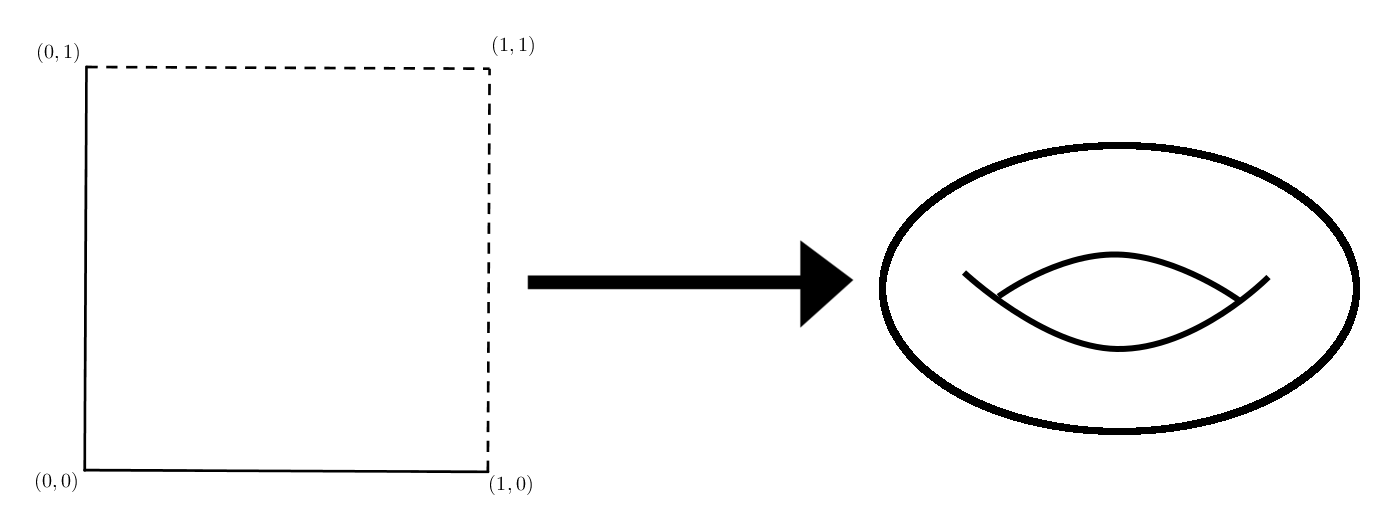
\includegraphics[width=0.7\linewidth]{images/frtorus}
	\caption{}
	\label{fig:frtorus}
\end{figure}

	

	
	

Open sets in the torus $\mathbb{R}$ are $\emptyset$ and $\mathbb{T}$, and the intersection of any standard open set with the fundamental region.  This is the same as the inherited subspace topology from $\mathbb{R}^2$.

\example{If we consider $\mathbb{R}^2/\mathbb{Z}$, where $a\in \mathbb{Z}$ acts on $\mathbb{R}^2$ by $a.(x,y)=(x+a,y)$.  A fundamental domain of this action is a vertical strip of unit width.  Again this inherits a subspace topology from $\mathbb{R}^2$.}



	







	\begin{figure}[!htb]
		\centering
		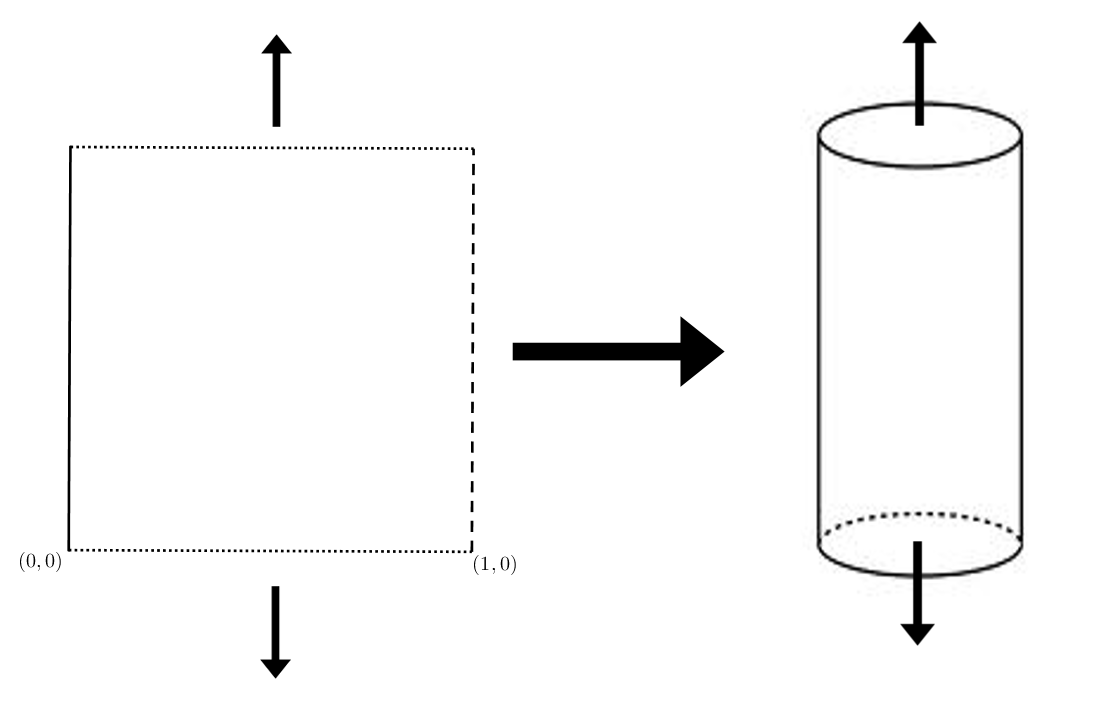
\includegraphics[width=0.7\linewidth]{images/frcyl}
		\caption{}
		\label{fig:frcyl}
	\end{figure}
	
	
	
	
	
\example{Consider again $\mathbb{R}^2/\mathbb{Z}$ but this time with the group action $a.(x,y)=(x+a,(-1)^ay)$.  The fundamental region is still a strip of unit width, but this time instead of identifying points on
	the boundary with their horizontal translation, we identify them with their horizontal translation
	composed with reflection about the $x$-axis. This space is homeomorphic to an infinite Moebius strip,
	which is difficult to draw.}


\example{Consider the equivalence relation on $\mathbb{R}^2$ described by $(x,y)\sim (x,y)$, $(0,y)\sim(1,y)$, and $(x,0)\sim(1-x,1)$.  The fundamental region again is a square with the left and right edges identified
	by simple translation, but the top and bottom edges are now identified by translation plus a flip
	across the square’s vertical axis of symmetry. This is homeomorphic to the Klein bottle, which is,
	again, hard to draw.}

\example{The previous example where we also identify the left and right edges by translation and
	a flip is called the real projective plane, denoted $\mathbb{R}P^2$
	. Both vertical and horizontal strips of this
	space look like Moebius strips. This is, once again, not easy to draw.}

\example{This one we can draw! Take the unit square as the fundamental region, but identify
	the top and left edge with each other by symmetry about the corner where they intersect, and do
	the same for the bottom and right edge. This space is homeomporhic to the 2-sphere $\mathbb{S}^2$
	.}
	
	
\begin{figure}[!htb]
\centering
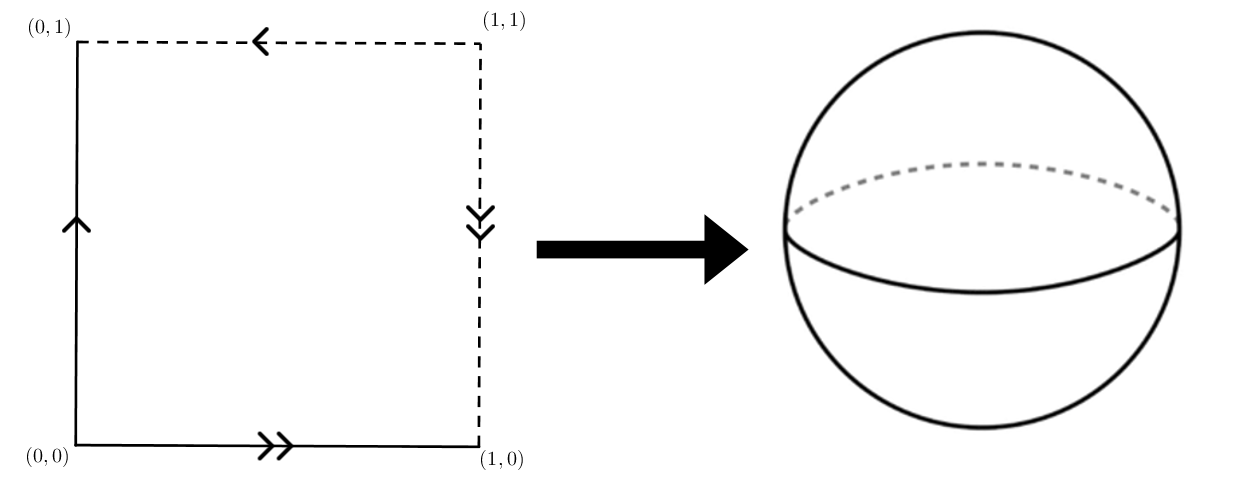
\includegraphics[width=0.7\linewidth]{images/frs2}
\caption{}
\label{fig:frs2}
\end{figure}
	
	
	
	


	\classheader{09-08-2017}


\section*{Mapping Cylinders and Tori}


\definition{Let $I$ denote the closed unit interval $[0,1]$.  The \textbf{mapping cylinder} of a continuous map $:fX\rightarrow Y$ is the quotient space defined by $X\times I/\sim$, where $(x,0)\sim (f(x),1)$.}


\definition{The \textbf{mapping torus} of a map $f:X\rightarrow X$ is similar, except that we require that the map be from a space to a copy of itself and we define the equivalence relation as $(x,0)\sim(f(x),0)$.}

\example{The mapping cylinder of $f:\mathbb{S}^1\rightarrow \mathbb{S}^1$ where $f(x)=x$ is a regular old cylinder.  The mapping torus is a regular old torus.}

\example{We can equivalently think of $\mathbb{S}^1$ as $\{ (x,y)|x^2+y^2=1 \}$ in Euclidean space or as $\{(r,\theta)|r=1  \}$ in polar coordinates.  Using this second formulation, consider the map $f:\mathbb{S}^1\rightarrow \mathbb{S}^1$ where $f(\theta)=2\theta$.  This is a two-to-one map which maps antipodal points to each other.  The mapping cylinder of $f$ is a Moebius strip.}

\example{What about the three-to-one map $f(\theta)=3\theta$?  The mapping cylinder of this looks like a three-bladed wing with a one-third twist and the ends glued together.}

\section*{Boundaries and Exteriors}

Let $(X,\mathcal{A})$ be a topological space and let $K\subseteq X$.

\definition{The \textbf{interior} of $K$ is the largest open subset contained in $K$.  That is, it is the union of all $U\subset K$ such that $U\in \mathcal{A}$.}

\definition{The \textbf{closure} of $K$ is the smallest closed subset containing $K$.  That is, it is the intersection of all $V\superset K$ such that $(X-V)\in \mathcal{A}$.}

\definition{The \textbf{boundary} of $K$ is the intersection of the closure of $K$ with the closure of the complement of $K$, that is $Bd(K) = \overline{K}\cap \overline{X-K}$.  If $K$ is open, then $Bd(K) = \overline{K}-K$.  If $K$ is closed, then $Bd(K)=\emptyset$.}


\example{Take $K = \mathbb{Q}\cap [0,1]\subset \mathbb{R}$ with the standard topology on $\mathbb{R}$.  The interior of this set is empty, as there is no open interval which doesn't contain an irrational number, so $\emptyset$ is the largest open subset in $K$.  The closure of $K$ is the entire interval $[0,1]$, as there is no smaller closed set which contains all of the rationals in that interval.  We also have that the boundary $Bd(K) = [0,1]$.}

\example{Take $K=\mathbb{R}-\{0\}$ with the Zariski topology on $\mathbb{R}$.  The interior of $K$ is $K$, as $K$ is open.  The closure of $K$ is all of $\mathbb{R}$, and the boundary is $\{0\}$.}

\definition{A point $x$ is a \textbf{limit point} of $K\subset X$ if every open set containing $x$ has non-empty intersection with $K$.  Equivalently, $x$ is a limit point of $K$ if $x\in \overline{K-\{x\}}$.}



\example{Take $\mathbb{R}$ with the Zariski topology.  If $U$ is an open set, then every $x\in\mathbb{R}$ is a limit point of $U$.  In fact, for any infinite subset of $\mathbb{R}$, every point in $\mathbb{R}$ is a limit point.}



	
	\classheader{09-11-2017}


\section*{Topological Bases}

\definition{Let $X$ be a set.  A collection $\mathcal{B}$ of subsets of $X$ is called a \textbf{base} (or \textbf{basis}) of $X$ if:
	
	\begin{enumerate}
		\item[1] If $x\in X$ then there is a $B\in \mathcal{B}$ such that $x\in B$.  Equivalently, $\mathcal{B}$ covers $X$.
		\item[2] If $B_1,B_2 \in \mathcal{B}$ and $x\in B_1\cap B_2$, then there is a $B_3\in\mathcal{B}$ such that $B_3\subset B_1\cap B_2$ and $x\in B_3$.
	\end{enumerate}
}

This is a weaker concept than a topology; we don't require that the union of base elements is a base element and we only require that the intersection of base elements contains another base element.

\example{Consider $\mathbb{R}^2$ with the standard topology.  Define $\mathcal{B} = \{ B_x(r) |x\in\mathbb{R}^2,r>0 \}$ as the set of open balls in $\mathbb{R}^2$. This is a base.  It is easy to see the first criterion is satisfied.  To see the second, consider two balls which both contain some point $x$.  Then there is a small ball centered at $x$ which is fully contained in the intersection of the two balls.  This smaller ball is also a base element, so we are done.}

\lemma{If $\mathcal{B}$ is a base and  $B_1,B_2,\dots,B_n \in \mathcal{B}$, and $x\in B_1\cap B_2\cap\dots\cap B_n$ then there exists a base element $B'\subset B_1\cap\dots\cap B_n$ which contains $x$.}

\begin{proof}
	We proceed by induction.  Since $x\in B_1\cap B_2$, there exists some $D_1\in\mathcal{B}$ such that $x\in D_1\subset B_1\cap B_2$.  Then $x\in D_1\cap B_3$, so there exists some $D_2\in\mathcal{B}$ with $x\in D_2$.  We proceed iteratively like this to find there is some $D_{n-1}\in \mathcal{B}$ with $x\in D_{n-1}$, and we set $B'=D_{n-1}$.
	
	
	
\end{proof}
	

\definition{A \textbf{topology generated by a base} is the collection of sets which are unions of base elements.}

If $X$ is a set with a base $\mathcal{B}$, then there is a smallest (coarsest) topology on $X$ containing $\mathcal{B}$, which is the topology generated by $\mathcal{B}$.  Open sets are the base elements, arbitrary unions of base elements, and $\emptyset$ and $X$ by definition.  Do we get the intersection property as well?

\claim{Yes.}

\begin{proof}
	If $B_1,\dots,B_n$ are base elements, then we can write the intersection $\bigcap\limits_{i\in [n]}B_i$ as the union of base elements just by taking neighborhoods of each point in the intersection.  If we have $U_1,\dots,U_n$ open in $X$ and $x\in \bigcap\limits_{i\in[n]}U_i$, then there is some base element in the intersection containing $x$.  If we do this for all points in the intersection, we can write the intersection as an arbitrary union of base elements, and we are done.
\end{proof}

\definition{Let $(X,\mathcal{A}$ be a topological space.  Take $\mathcal{B}\subset \mathcal{A}$ a collection of sets such that $\emptyset,X\in \mathcal{B}$ and if $x\in U\in \mathcal{A}$, then there is some $B\in\mathcal{B}$ such that $x\in B\subset U$.  We call $\mathcal{B}$ a \textbf{base for the topology $\boldsymbol{\mathcal{A}}$}.}


	
	\end{document}
	
